Kontrol limitleri için daha önceden hesapladığımız ortalama örneklem standart sapması ve n=5 için olan katsayıları kullanarak hesaplama yapıldığında: 

\begin{itemize}
	\centering
	\item 
	$UCL=B_4 \bar{s}=(2,089 \cdot 0,1757)=0,3671$
	\item
	$CL=\bar{s}=0,1757$
	\item
	$LCL=B_3 {s}=(0 \cdot 0,1757)=0$
\end{itemize}


Süreç aslında “istatistiksel olarak kontrol altındadır” ama incelenilmesi gereken bazı noktalar vardır.\\

S Kontrol Kart'ı tıpkı $\bar{X}$ Kontrol Kartı'nda da söylendiği gibi operatör farklılıkları, makine kalibre sıkıntıları, standartize edilmemiş üretim gibi sorunlara sahip olabilir. Ayrıca bu grafik, yapılan her bir gözlemdeki ürünlerin gramaj değişikliğin kontrol limitlerinin altında dahi olsa süreçteki bir düzensizliği ortaya koymaktadır.\\

Bu süreç özelinden gidildiğinde $\bar{X}$ Kontrol Kartı ile S Kontrol Kartları'nın en büyük farkı ise, birisinin her bir gözlemdeki “ortalamamız ne?” sorusuna cevap vermeye çalışırken diğerinin ise her bir gözlemde “tutarlılığımız ne kadar?”  sorusuna cevap vermeye çalışmasıdır. \\

Bir örnek ile anlatılmak istenilirse, 2 kiloluk ürün ile 10 kiloluk ürünün ortalaması 6 kilodur fakat 5 kiloluk ve 7 kiloluk iki ürününde ortalaması da 6 kilo olacaktır. İki durumu birbirinden ayırabilmek ve sürecin tutarlı, ürünlerin aynı kalitede olabilmesi için gözlemlerin standart sapmalarının düşük olmasını beklemek kesinlikle normal ve istenilmesi gerekilen bir durumdur.\\

\begin{figure}[ht]
	\centering
	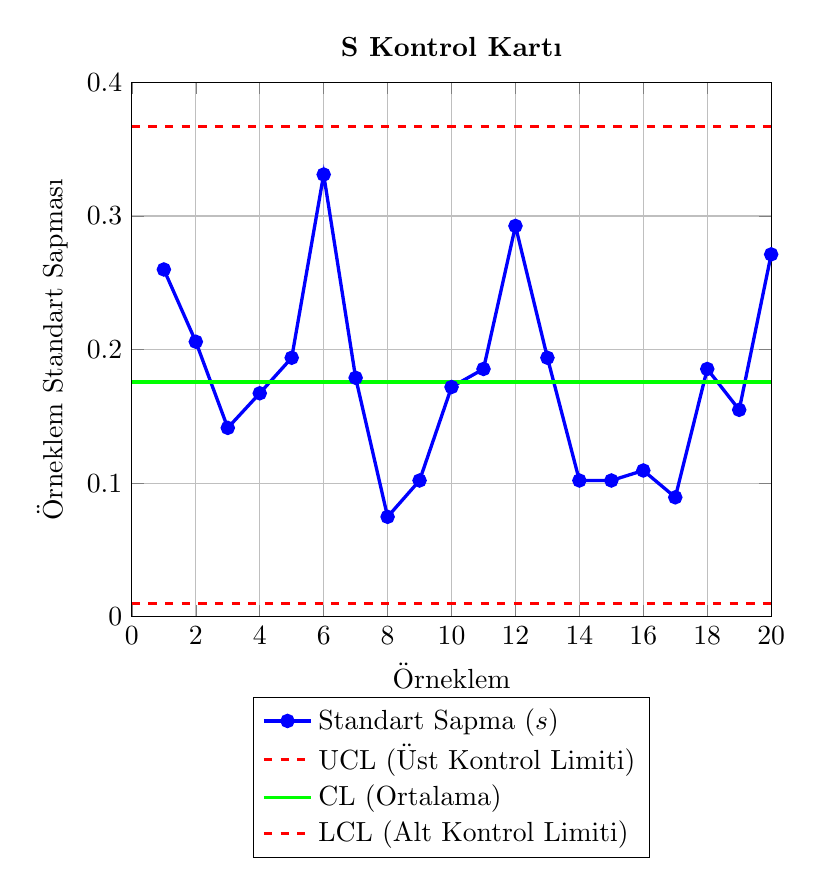
\begin{tikzpicture}
		\begin{axis}[
			title={\bfseries S Kontrol Kartı},
			xlabel={Örneklem},
			ylabel={Örneklem Standart Sapması},
			xmin=0, xmax=20,
			ymin=0, ymax=0.4,
			grid=both,
			yticklabel style={/pgf/number format/fixed},
			legend style={at={(0.5,-0.15)}, anchor=north}, % legend'ı alt tarafa yerleştirme
			legend cell align=left,
			legend entries={},
			width=0.8\textwidth
			]
			% Standart Sapma (s) verisi
			\addplot[
			color=blue,
			mark=*,
			very thick
			] coordinates {
				(1, 0.26) (2, 0.2059) (3, 0.1414) (4, 0.1673) (5, 0.1939) 
				(6, 0.3311) (7, 0.1789) (8, 0.0748) (9, 0.1020) (10, 0.1720)
				(11, 0.1855) (12, 0.2926) (13, 0.1939) (14, 0.1020) (15, 0.1020) 
				(16, 0.1095) (17, 0.0894) (18, 0.1855) (19, 0.1549) (20, 0.2713)
			};
			\addlegendentry{Standart Sapma ($s$)}
			
			% UCL çizgisi
			\addplot[
			color=red,
			dashed,
			very thick
			] coordinates {
				(0, 0.3671) (20, 0.3671)
			};
			\addlegendentry{UCL (Üst Kontrol Limiti)}
			
			% CL çizgisi
			\addplot[
			color=green,
			very thick
			] coordinates {
				(0, 0.1757) (20, 0.1757)
			};
			\addlegendentry{CL (Ortalama)}
			
			% LCL çizgisi
			\addplot[
			color=red,
			dashed,
			very thick
			] coordinates {
				(0, 0.0100) (20, 0.0100)
			};
			\addlegendentry{LCL (Alt Kontrol Limiti)}
			
		\end{axis}
	\end{tikzpicture}
	\caption*{}
\end{figure}


Ödevin bu kısmına kadar yapılan (a) şıkkının S Kontrol Kartı'nın yorumlaması yapıldıktan sonra artık (b) şıkkı hakkında yorumlamalar yapılacaktır.

\cleardoublepage

